%%
%%  This is a LaTeX template for an astronomy Bachelor's thesis.
%%
%%  Version 1.0
%%
%%  Authors: Anders Johansen, Sofia Feltzing, Johan Bijnens (2014)
%%  Send feedback to Anders Johansen <anders@astro.lu.se>
%%
\documentclass[12pt]{report}

\usepackage{a4wide}
\usepackage{graphicx}
\usepackage{natbib}
\usepackage[T1]{fontenc}  
\usepackage[utf8]{inputenc} 
\usepackage{geometry}
\usepackage{caption}
\usepackage{subcaption}

\usepackage{fancyhdr}
\usepackage{lastpage}
\usepackage{pdfpages}
\usepackage{url}

\pagestyle{fancy}
%\rhead{}
%\chead{}
%\lhead{}
%\rfoot{}
\cfoot{\thepage}
%\lfoot{}

\newcommand{\apj}{ApJ}
\newcommand{\apjl}{ApJ}
\newcommand{\mnras}{MNRAS}
\newcommand{\aap}{A\&A}
\newcommand{\aj}{AJ}
\newcommand{\nat}{Nature}
\newcommand{\pre}{Phys.~Rev.~E}
\newcommand{\araa}{ARA\&A}
\newcommand{\icarus}{Icarus}

\begin{document}

\title{\huge \bf A LaTeX template for an astronomy/astrophysics
thesis\footnote{This is just a very basic cover page produced by LaTeX -- when
the thesis is done you can get a more formal cover page from Eva Jurlander.}}
\author{Lucas Hellström}

\thispagestyle{empty} % do not count pages just yet

\maketitle

\newpage

\thispagestyle{empty}

\begin{center}
  (this page will contain some more official information in the final version)
\end{center}

\newpage

\thispagestyle{empty}

\begin{center}
  {\bf Abstract}
\end{center}
The abstract is a short summary describing the content of the main text. This
should give enough information about the contents to decide for the intended
audience whether further reading will be useful. The size should be about half
a page, best written at the end, after most of the thesis is written.

\newpage

\thispagestyle{empty}
\mbox{} % this is how we create an empty page in LaTeX

\newpage

\thispagestyle{empty}

\begin{center}
  {\bf Popul\"arvetenskaplig beskrivning}
\end{center}
This is meant to be popular {\it introduction to} and {\it description of} your
thesis, preferably written in Swedish. The name is unfortunately misleading. It
is not a summary but mainly an introduction to what you have done. A good idea
is to write this when you are about one third through the time allotted for the
thesis work.
\\ \\
Especially important here are the context of your project and why this is an
interesting project to do. This should be about half a page as well.
% Swedish letters: \"a, \"o, \aa

\newpage

\thispagestyle{empty}
\mbox{} % make sure that TOC starts on a right page

\newpage

\setcounter{page}{1} % start counting pages

\tableofcontents

\newpage

\listoffigures 
\listoftables

\newpage

\chapter{Introduction}

This document is meant as a technical tutorial for writing an
astronomy/astrophysics thesis in LaTeX. Detailed rules about the {\it contents}
of the thesis (Bachelor's thesis or Master's thesis) can be found at the course
websites.

\section{TESS}


\section{Transits}

\subsection{Variations}

\section{Simulation of TESS objects}

\section{TTVFast}

\section{Analyzing results from TTVFast}



\chapter{Results}

Chapters always start on a new page. The chapter names in the template are just
suggestions. You can name your chapters differently and add more if needed.

\section{Code}

When we write down computer code we might want it to look just like it does in
the editor (using a fixed with font). This is done using the {\sl verbatim}
environment.

\begin{verbatim}

       PROGRAM myfortran

       IMPLICIT NONE

       REAL*8 mag(20)
       REAL flux(20)
       INTEGER nstar

       WRITE(*,*) "This program calculates a magnitude"
       READ(*,*) flux(1)
       mag(1)=-2.5*LOG(flux(1))

\end{verbatim}

\section{Figures}

Figures are of course very important in the thesis. Make sure that your figures
have thick lines that stand out in the printed version, that the fonts are not
too small, that the axes are labelled and explained and that colours are
distinguishable in a black and white printout as well (this is helpful for the
not insignificant fraction of the population who are colorblind).
\begin{figure}
		\centering
		\begin{minipage}{.5\textwidth}
 		 \centering
 		 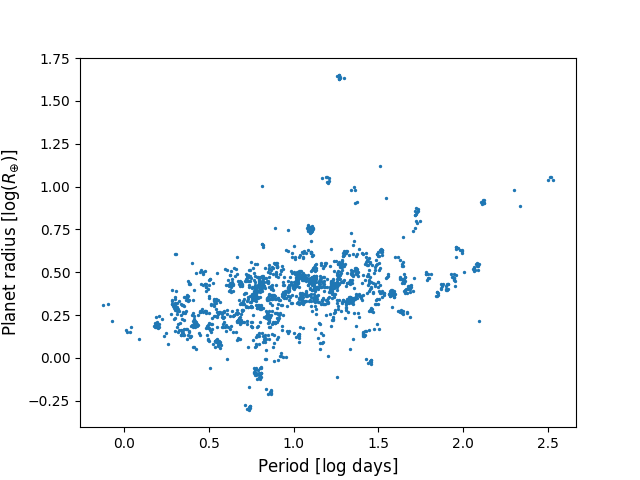
\includegraphics[width=8cm]{img/R_P-plot_5.png}
 		 \captionof{figure}{Diagram with the radius \\distribution as a function of period for\\ the simulated TESS objects.}
 		 \label{fig:start}
		\end{minipage}%
		\begin{minipage}{.5\textwidth}
 		 \centering
		  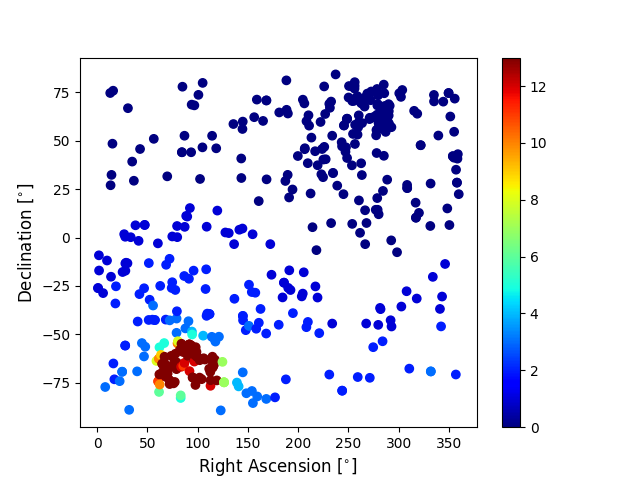
\includegraphics[width=8cm]{img/RA_Dec_Max.png}
		  \captionof{figure}{Diagram with the position of each observed objects color-coded to show the number of times the object is observed.}
		  \label{fig:saturation}
		\end{minipage}
	\end{figure}

\section{Tables}

This section contains a table which shows the most basic elements and a simple
layout. The table can be seen in Table\,\ref{table:1}.  Make sure to make your
labeling system easy. Maybe table:1 is not so smart -- what if you move the
table somewhere else, and it is not any longer the first table or you add a
table before this one. A label like {\tt table:varstars} is much better.
\begin{table}[!h]
\caption{This is a table of variable stars}\smallskip
\label{table:1}
\centering  
\begin{tabular}{lrrc}
\hline\hline  
\smallskip
Id of star & I &  V & Var.? \\
\hline
1234 & 15.6 & 17.3 & No \\
5677 & 13.4 & 12.3 & Yes\\
\hline
\end{tabular}
\end{table}
\\ \\
Here we managed to place the table directly in the text (using the !h option).
Generally we should let LaTeX control the positions of figures and tables --
if you are unhappy with their placement then try to move them around in the raw
text or experiment with !h and !t.

\section{Equations}

Writing mathematical formulae in LaTeX is not always so easy at first. But it
does look good! This is one of the main reasons why we use LaTeX instead of
Word. There are several environments that we can use. If I want simply to have
a small equation or some expression in the text I can just do {\tt \$ x+a
\textbackslash cdot b= f(x) \$}. Which, when LaTeXed, gives us the formula $x+a
\cdot b= f(x)$.
\\ \\
If we want an equation by itself, we just add one more {\tt \$} at each side:
$$ g(x,y)=\sin (x) + 10 \ log(y \cdot 20 \cdot 10^{-2x}) $$
It is also possible to use an {\sl environment} especially for equations.
Remember that equations should be integrated in the flow of the text, even if
they are on separate lines. Therefore we should use punctuation in equations as
well, for example in the equation which reads
\begin{equation}
  \sum_{k=i}^n (x- \overline{x})^2 +\sqrt{x^2 + y^3} = h(x,y) \label{eq:smart}
  \, .
\end{equation}
\\ \\
Remember that the {\sl equation} environment does not like empty lines.  This
is the same in table, by the way.  You can do many more things in the
maths-mode. If you are going to write lots of equations you will learn it very
quickly.

\section{The list environment}

If you want to make good looking lists, short or long, LaTeX can do it for you.

\begin{itemize}
\item This is the first entry
\item and the second one
  \begin{itemize}
    \item lets go down one level
    \item and stay there
      \begin{itemize}
          \item And one more
          \item very deep
      \end{itemize}
  \end{itemize}
\end{itemize}

But you can also do other types of lists. For example with numbers. Very useful
as you cna refer to them later.

\begin{enumerate}
  \item First entry
  \item Second entry
  \item Third entry
    \begin{enumerate} 
  \item First entry \label{label:item}
  \item Second entry
  \end{enumerate}
      \begin{itemize}
          \item And you can mix the listings
          \item like this 
      \end{itemize}
\end{enumerate}     

\chapter{Conclusions}

\section{Cross-referencing}

LaTeX is very nice because it can help you to refer to the right table, figure,
item section or page. Just remember that you need to compile with {\tt latex}
or {\tt pdflatex} twice (!) before it has updated all the cross references.
This is also true for references (see Sect.\,\ref{sect:refs}).
\\ \\
In item\,\ref{label:item} on page \pageref{label:item} you can find some
important information that was not covered in Eq.\,(\ref{eq:smart}) or in
Table\,\ref{table:1}. That covers the most important references.

\section{References}
\label{sect:refs}

You also need to cite all the thick and good papers that you have read during
your thesis work. There are several ways. Here we will use the {\tt natbib}
style as that one is the one that most resembles the way we write references in
astronomy journal papers. 
\\ \\
You can add the references in a so called bibtex file. This file contains all
the information LaTeX needs about a single paper in order to make an entry in
the reference list and to write the correct reference inside your text. You can
go to ADS and download references and add them to the bibtex file. Click
on the link marked ``Bibtex entry for this abstract" and paste the entry into
the bibtex file. You can then compile the document with {\tt latex
thesis\_template}, {\tt bibtex thesis\_template}, {\tt latex thesis\_template},
{\tt latex thesis\_template}.
\\ \\
Alternatively we can add a list of bibitems directly in the LaTeX file. On ADS,
click instead on the link marked ``Preferred format for this abstract" and
paste the bibitem into the reference list. This method is included in the
template but is commented out. If you use bibitems then you can compile the
document by simply typing {\tt latex thesis\_template} twice.
\\ \\
Both methods allow you to cite the important paper by
\cite{2007MNRAS.375..500A} which was based on earlier work
\citep{2001A&A...373.1019S}.

\section{Spelling}

Remember to check the text carefully for typos and grammatical errors. You can
use a tool like Spell Right for this
(\url{http://nile.lub.lu.se/loDownload/101/Spellright.htm}) -- but note that
you must paste the text into a Word file in order to feed it into Spell Right.

\section*{Acknowledgements}

There is no acknowledgements section in the regular LaTeX, but you can easily
make one yourself. \citep{2017A&A...598L...7K}

%\bibliographystyle{natbib}
%\begin{thebibliography}{99}
%\bibitem[Alexander \& Armitage(2007)]{2007MNRAS.375..500A}
%  Alexander, R.~D., \& Armitage, P.~J. 2007, \mnras, 375, 500
%\bibitem[Santos et~al.(2001)Santos, Israelian, \& Mayor]{2001A&A...373.1019S}
%  Santos, N.~C., Israelian, G., \& Mayor, M. 2001, \aap, 373, 1019
%\end{thebibliography}

\bibliographystyle{aa}
\bibliography{references}

\begin{appendix}

\chapter{This is an appendix}

You can put long mathematical derivations or tables in appendices.

\chapter{This is another appendix}

\begin{verbatim}
	import matplotlib.pyplot as plt
import numpy as np
import sys

timesFile = []
valueArray = []
transitTime1Float = []
epoch1Float = []
count = 0
period = 1.0917340278625494e+01
kepMag = []
transitDur = []
rStar = []

with open(sys.argv[1],'r') as timesFile:
	valueArray = timesFile.readlines()
	planet = [k.split(' ')[0] for k in valueArray]
	epoch1 = [k.split(' ')[1] for k in valueArray]
	transitTime1 = [k.split(' ')[2] for k in valueArray]


for k in range(len(valueArray)):
	if planet[k] == '0':
		epoch1Float.append(float(epoch1[k]))
		transitTime1Float.append(float(transitTime1[k]))

epoch1Float = np.array(epoch1Float)
transitTime1Float = np.array(transitTime1Float)

transitTime1Min = transitTime1Float * 1440
fitTimes = np.polyfit(epoch1Float, transitTime1Min, 1)

transitTimesLinFitted = transitTime1Min-fitTimes[0]*epoch1Float
transitMax = np.amax(transitTimesLinFitted)
transitMin = np.amin(transitTimesLinFitted)
transitAmplitude = (transitMax - transitMin) / 2
transitCorrection = (transitMax + transitMin) / 2

outputFile = open('transAmpl.txt', 'a')
outputFile.write(repr(transitAmplitude) + '\n')

print "Amplitude:", transitAmplitude, "minutes or", transitAmplitude/60, "hours"

if transitMax < 0:
	transitTime1Corrected = transitTimesLinFitted + abs(transitCorrection)
else:
	transitTime1Corrected = transitTimesLinFitted - abs(transitCorrection)

with open('timingErrors.csv','r') as inputFile:
	data = inputFile.readlines()[0:]
	errorTiming = float(data[int(sys.argv[2])])


plt.scatter(epoch1Float*fitTimes[0]/1440, transitTime1Corrected, label='Transit Time')
plt.errorbar(epoch1Float*fitTimes[0]/1440, transitTime1Corrected, yerr = errorTiming, linestyle="None")
plt.xlabel('Time [Days]')
plt.ylabel('Transit time [Minutes]')
plt.title('Transit Timing variations')
plt.legend()
plt.tight_layout()
textstr = 'Amplitude=%.2f\nError=%.2f\n'%(transitAmplitude, errorTiming)
plt.figtext(0.75, 0.5, textstr, fontsize=10)
plt.subplots_adjust(right=0.7)
plt.savefig('plots/' + sys.argv[1] + '.png')
\end{verbatim}
\end{appendix}

\end{document}
